\chapter{Marktsegmente}
Im Kapitel Marktsegmente werden die aktuellen Bereiche von Internet of Things, Smartwatches und Smartwatches im Internet of Things aufgezeigt. Es werden nur Bereich aufgezeigt in welchen die erwähnten Themen eine Rolle spielen. Es wird keine strategische Marktsegmentierung durchgeführt.

\section{Marktsegmente im Internet of Things}
\begin{tabbing}
xxxxxxxxxxxxxxxxxxxx\=xxxxxxxxxxxxxxxxxxxxxxxx	\kill
Industrie:  		 \>  Maschinensteuerung, Automatisierte Roboter, Lagerüberwachung \\
Automobil: 		   \>  Telemetrie, Geografische Strecke, Fahrverhalten, Nutzungsverhalten, Verkehrsbericht \\
Städte{/}Verkehr:\>  Touristisches Informationen, Dynamische Strassen, Verkehrsregulierung, Navigation, Lageberichte \\
Heimautomation:	 \>  Nutzung und Überwachung von Haushaltsgeräte, Steuerung, Fernbedienungen \\
Detailhandel:		 \>  Produktebezeichnung, Kasse, Geldüberweisung, Geldbörse \\
Mensch:          \>  Blutdruck, Puls, Bewegungen, Schlaf Überwachung, \\\>Körperanalyse {(z.B. Gewicht, Fettanteil, Wasseranteil usw.)} \\
Natur:			     \>  Erdplatten Bewegung, Wasserspiegel Überwachung, Temperatur, Wind, Licht, Luft \\\\

Wie in der Tabelle aufgelistet, kommt das Internet der Dinge in sehr vielen verschiedenen Marktsegmenten zum tragen.\\
Es hat noch grösseres Potential den Mensch zu unterstützen und ihre Aufgaben zu erleichtern, als es jetzt schon tut.
\end{tabbing}

\subsection{Industrie}
Das Internet der Dinge kommt in der Industrie soweit zum tragen, dass man von Industrie 4.0 spricht. Dies soll die vierte industrielle Revolution zum Ausdruck bringen. Die Fertigungstechnologie soll informatisiert werden. Auch die Logistik soll ihre Automatisierung erleben. Erreicht wird dies weil Maschinen untereinander kommunizieren können. Die Abbildung 3.1 illustriert symbolisch die Vernetzung aller Sektoren einer Fabrik. Das Ziel der Industrie 4.0 ist die intelligente Fabrik.
\begin{figure}[h]
  \centering
  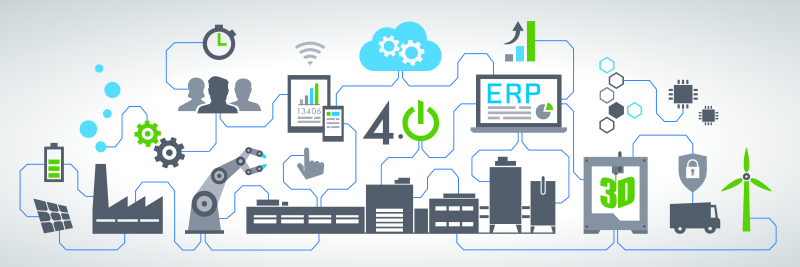
\includegraphics[scale=0.62]{98_Bilder/03_Marktsegmente/industrie4}
  \caption[Industie 4.0 Symbolbild]{Industie 4.0}
  \footnotesize Quelle: \url{https://www.scopevisio.com/ratgeber/wp-content/uploads/2015/11/Industrie-4.0.png}, Stand: 05.11.2015
\end{figure}
\newpage

\subsection{Automobil}
IoT kann in vielen Bereichen der Automobilbranche eingesetzt werden. Es können wichtige Daten des Fahrzeugs ausgelesen werden, z.B. die Telemetriedaten. Diese können dann verwendet werden um das Fahrvehalten vom Lenker festzustellen. Desweiteren können diese auch benutzt werden um Probleme beim Auto auszumachen und direkt Fahrer und Mechniker zu alarmieren.
Interessant, für die Autobauer wie auch Autobesitzer, ist auch die Ortung der Fahrzeuge. Mit den aufgezeichneten geografischen Punkte kann analysiert werden, wie das Automobil verwendet wird und aktuelle verkehrsnahe Verkersberichte können genutzt werden. Die Vollendung der Vernetzung von Fahrzeugen ist das selbstfahrende Auto, welches alle nötigen Informationen empfängt, analysiert und verwendet um das Ziel zu erreichen.\\
Mercedes-Benz hat ein selbstfahrendes Forschungsfahrzeug entwickelt (Siehe Abbildung 3.2). Die Abbildung 3.3 zeigt wie das Fahrzeug durch die Sensoren einen Fussgänger erkennt und die Laserprojektionstechnik als Aktor verwendet, um dem Überquerenden die Fussgängerstreifen aufzuzeigen.
\begin{figure}[h]
  \centering
  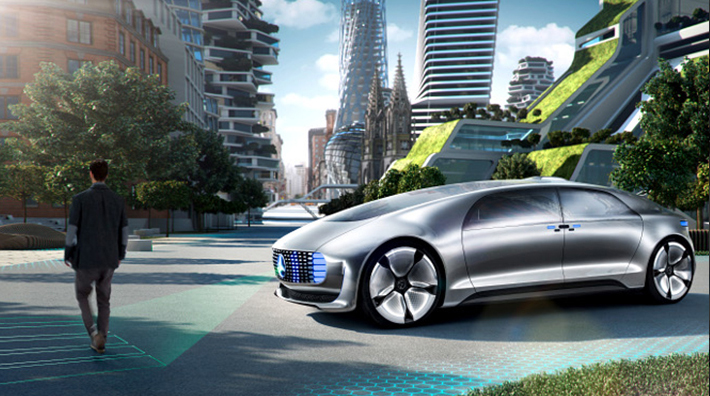
\includegraphics[scale=0.66]{98_Bilder/03_Marktsegmente/mercedesbenzf}
  \caption[Selbstfahrendes Auto Mercedes-Benz F015 In Motion]{Das selbstfahrende Forschungsfahrzeug von Mercedes-Benz (Modell F015 In Motion)}
  \footnotesize Quelle: \url{http://www.mercedes-benz.ch/content/media_library/.../f_015_luxury_in_motion_layer-gallery_1_01__710x396_01-2015.jpg}, Stand: 05.11.2015
  \centering
  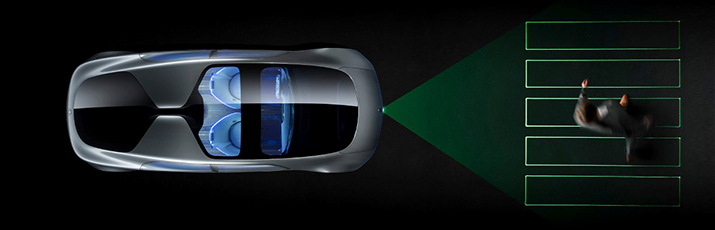
\includegraphics[scale=0.66]{98_Bilder/03_Marktsegmente/mercedesbenzf2}
  \caption[Fussgängererkennung des F015]{F015 In Motion erkennt Fussgänger mit seinen Sensoren}
  \footnotesize Quelle: \url{http://www.mercedes-benz.ch/content/media_library/.../f_015_luxury_in_motion_gallery_05_715x230_01-2015.jpg}, Stand: 05.11.2015
\end{figure}
\newpage

\subsection{Städte und Verkehr}
In Städten gibt es sehr viele Möglichkeiten, in Verbindung mit dem Verkehr geht dies ins unermessliche.
Ein sehr interessantes Thema ist die Touristik. Um ein Beispiel zu nennen, Beacons welche nötige Information an ein Smartgerät publizieren um Daten von der Sehenswürdigkeit abzurufen. Dazu könnte auch gleich Empfehlungen in der Umgebung notifiziert werden. So würde für die meisten Reisenden der Reiseführer wegfallen.

Ein spektakuläres Projekt ist die dynamische Strasse: \textbf{Solar Roadways}.\\
Das sind kleine, feste Platten mit Photovoltaik-Elementen, Elektronik, verschiedenen Sensoren und LEDs integriert (Siehe Abbildung 3.4). Die Platten können wie Pflastersteine verlegt und miteinander verbunden werden. Durch die Sonneneinstrahlung sind sie permanent und umweltschonend mit Strom versorgt. Die LEDs können zentral gesteuert werden, um so die Fahrbahnmarkierungen anzuzeigen und z.B. aus zwei breiten Spuren drei schmale zu machen oder spontane Parkflächen oder Verkehrszeichen oder was auch immer. Die Sensoren können feststellen, wenn Tiere darüber laufen und die Fahrer blitzschnell schon ein paar hundert Meter vorher über die LEDs warnen.  Und die Platten sind beheizbar. Kein tonnenweises Ausbringen von Streusalz mehr, keine Glatteisunfälle mehr, keine Asphalterneuerungen mehr und vermutlich viel weniger Baustellen. Einfach die defekten Platten austauschen, fertig. Das ist echte Innovation! Und das Beste daran: es ist von Privatpersonen initiiert und sogar crowdfunded. Das Vorhaben ist auf Indiegogo (\url{www.indiegogo.com}) im Juni 2014 deutlich überfinanziert abgeschlossen worden. Statt der benötigten eine Million US Dollar, sind über zwei Millionen US Dollar zusammengekommen. Die Holländer haben im Jahr 2014 bereits angefangen, Radwege auf diese Weise zu bauen. Die Fahrradwege über(Siehe Abbildung 3.5 und 3.6).\footnote{Quelle: \url{https://www.holisticon.de/2014/11/die-sache-mit-dem-horizont-iot-blogserie-episode-5}, Stand: 05.11.2015}
\begin{figure}[h]
  \centering
  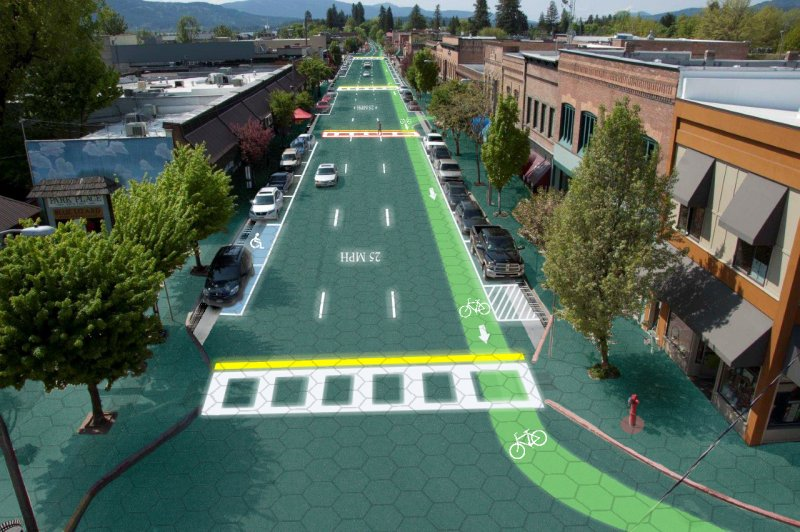
\includegraphics[scale=0.61]{98_Bilder/03_Marktsegmente/solar_roadway_00}
  \caption[Solar Roadway, dynamische Strasse]{Das Solar Roadway verändert die Strasse für die aktuelle Verkehrsituation}
  \footnotesize Quelle: \url{http://www.solarroadways.com/images/intro/Downtown%20Sandpoint%202%20-%20small.jpg}, Stand: 05.11.2015
\end{figure}
\newpage
\begin{figure}[H]
  \centering
  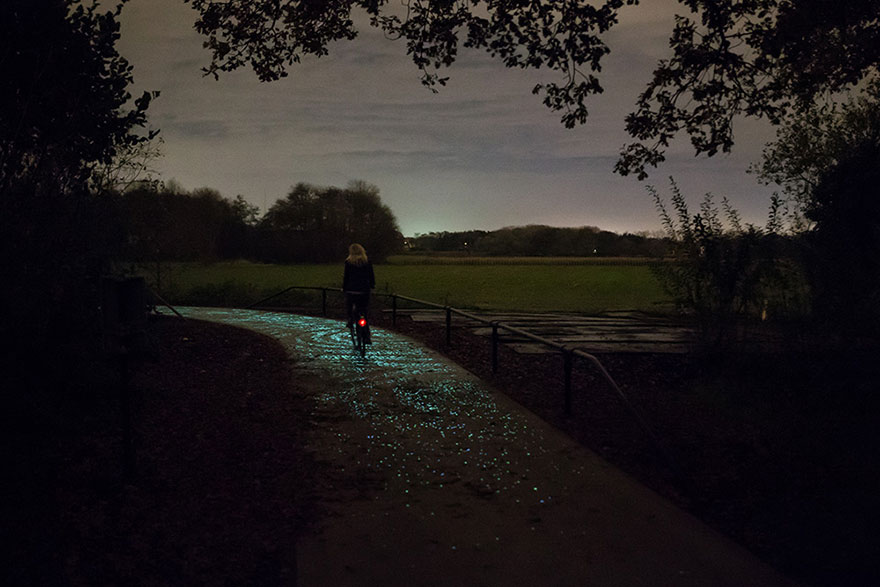
\includegraphics[scale=0.5]{98_Bilder/03_Marktsegmente/solar_roadway_02}
  \caption[Solar Roadway in der Dämmerung]{Solar Roadway: In der Dämmerung wird der Weg an den nötigen Stellen beleuchtet}
  \footnotesize Quelle: \url{http://static.boredpanda.com/blog/wp-content/uploads/2014/11/van-gogh-starry-night-glowing-bike-path-daan-roosengaarde-2.jpg}, Stand: 05.11.2015
  \centering
  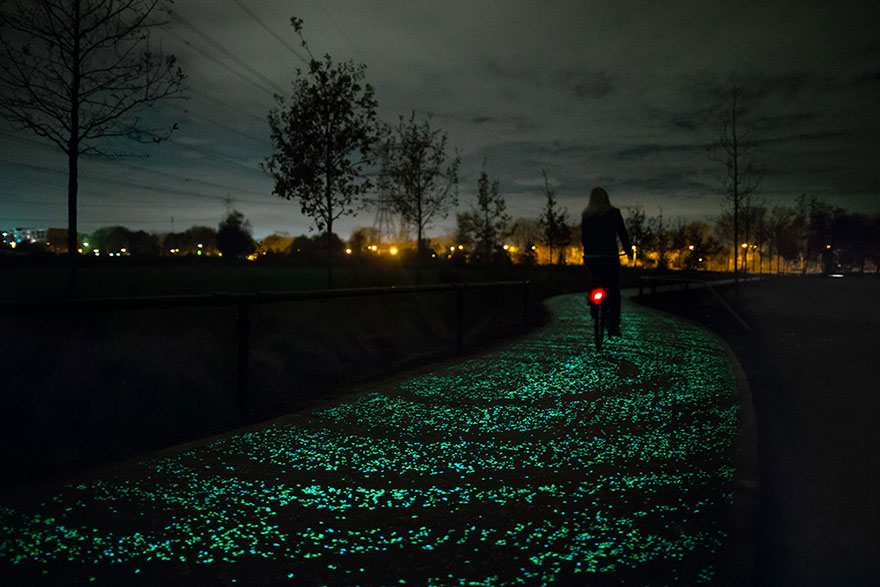
\includegraphics[scale=0.5]{98_Bilder/03_Marktsegmente/solar_roadway_01}
  \caption[Solar Roadway bei Nacht]{Solar Roadway: Bei Nacht ist der Veloweg komplett beleuchtet}
  \footnotesize Quelle: \url{http://static.boredpanda.com/blog/wp-content/uploads/2014/11/van-gogh-starry-night-glowing-bike-path-daan-roosengaarde-1.jpg}, Stand: 05.11.2015
\end{figure}
\newpage

\subsection{Heimautomation}
Die Heimautomation ist auch besser bekannt als Smart Home. Smart Home dient als Oberbegriff für technische Verfahren und Systeme in Wohnräumen und -häusern, in deren Mittelpunkt eine Erhöhung von Wohn- und Lebensqualität, Sicherheit und effizienter Energienutzung auf Basis vernetzter und fernsteuerbarer Geräte und Installationen sowie automatisierbarer Abläufe steht.

Unter diesen Begriff fällt sowohl die Vernetzung von Haustechnik und Haushaltsgeräten (zum Beispiel Lampen, Jalousien, Heizung, aber auch Herd, Kühlschrank und Waschmaschine), als auch die Vernetzung von Komponenten der Unterhaltungselektronik (etwa die zentrale Speicherung und heimweite Nutzung von Video- und Audio-Inhalten).

Von einem Smart Home spricht man insbesondere, wenn sämtliche im Haus verwendeten Leuchten, Taster und Geräte untereinander vernetzt sind, Geräte Daten speichern und eine eigene Logik abbilden können. Geräte sind teilweise auch getagged, was bedeutet, dass zu den Geräten im Smart Home Informationen zum Beispiel über Hersteller, Produktnamen und Leistung hinterlegt sind. Dabei besitzt das Smart Home eine eigene Programmierschnittstelle, die (auch) via Internet angesprochen und über erweiterbare Apps gesteuert werden kann.

Eng verwandt mit diesen Verfahren und Systemen sind solche des Smart Metering, bei denen der Schwerpunkt auf dem Messen und einer intelligenten Regulierung des Energieverbrauchs liegt.

Neben „Smart Home“ haben sich Begriffe wie Intelligentes Wohnen, „eHome“, „Smart Living“ und weitere Bezeichnungen etabliert, die sich teils nur in Bedeutungsschattierungen unterscheiden. Zudem verwenden Hersteller von Smart-Home-Anlagen und -komponenten weitere, speziell auf deren individuelles Marketing abgestimmte Begriffe.\footnote{Quelle: \url{https://de.wikipedia.org/wiki/Smart_Home}, Stand: 05.11.2015}
\begin{figure}[h]
  \centering
  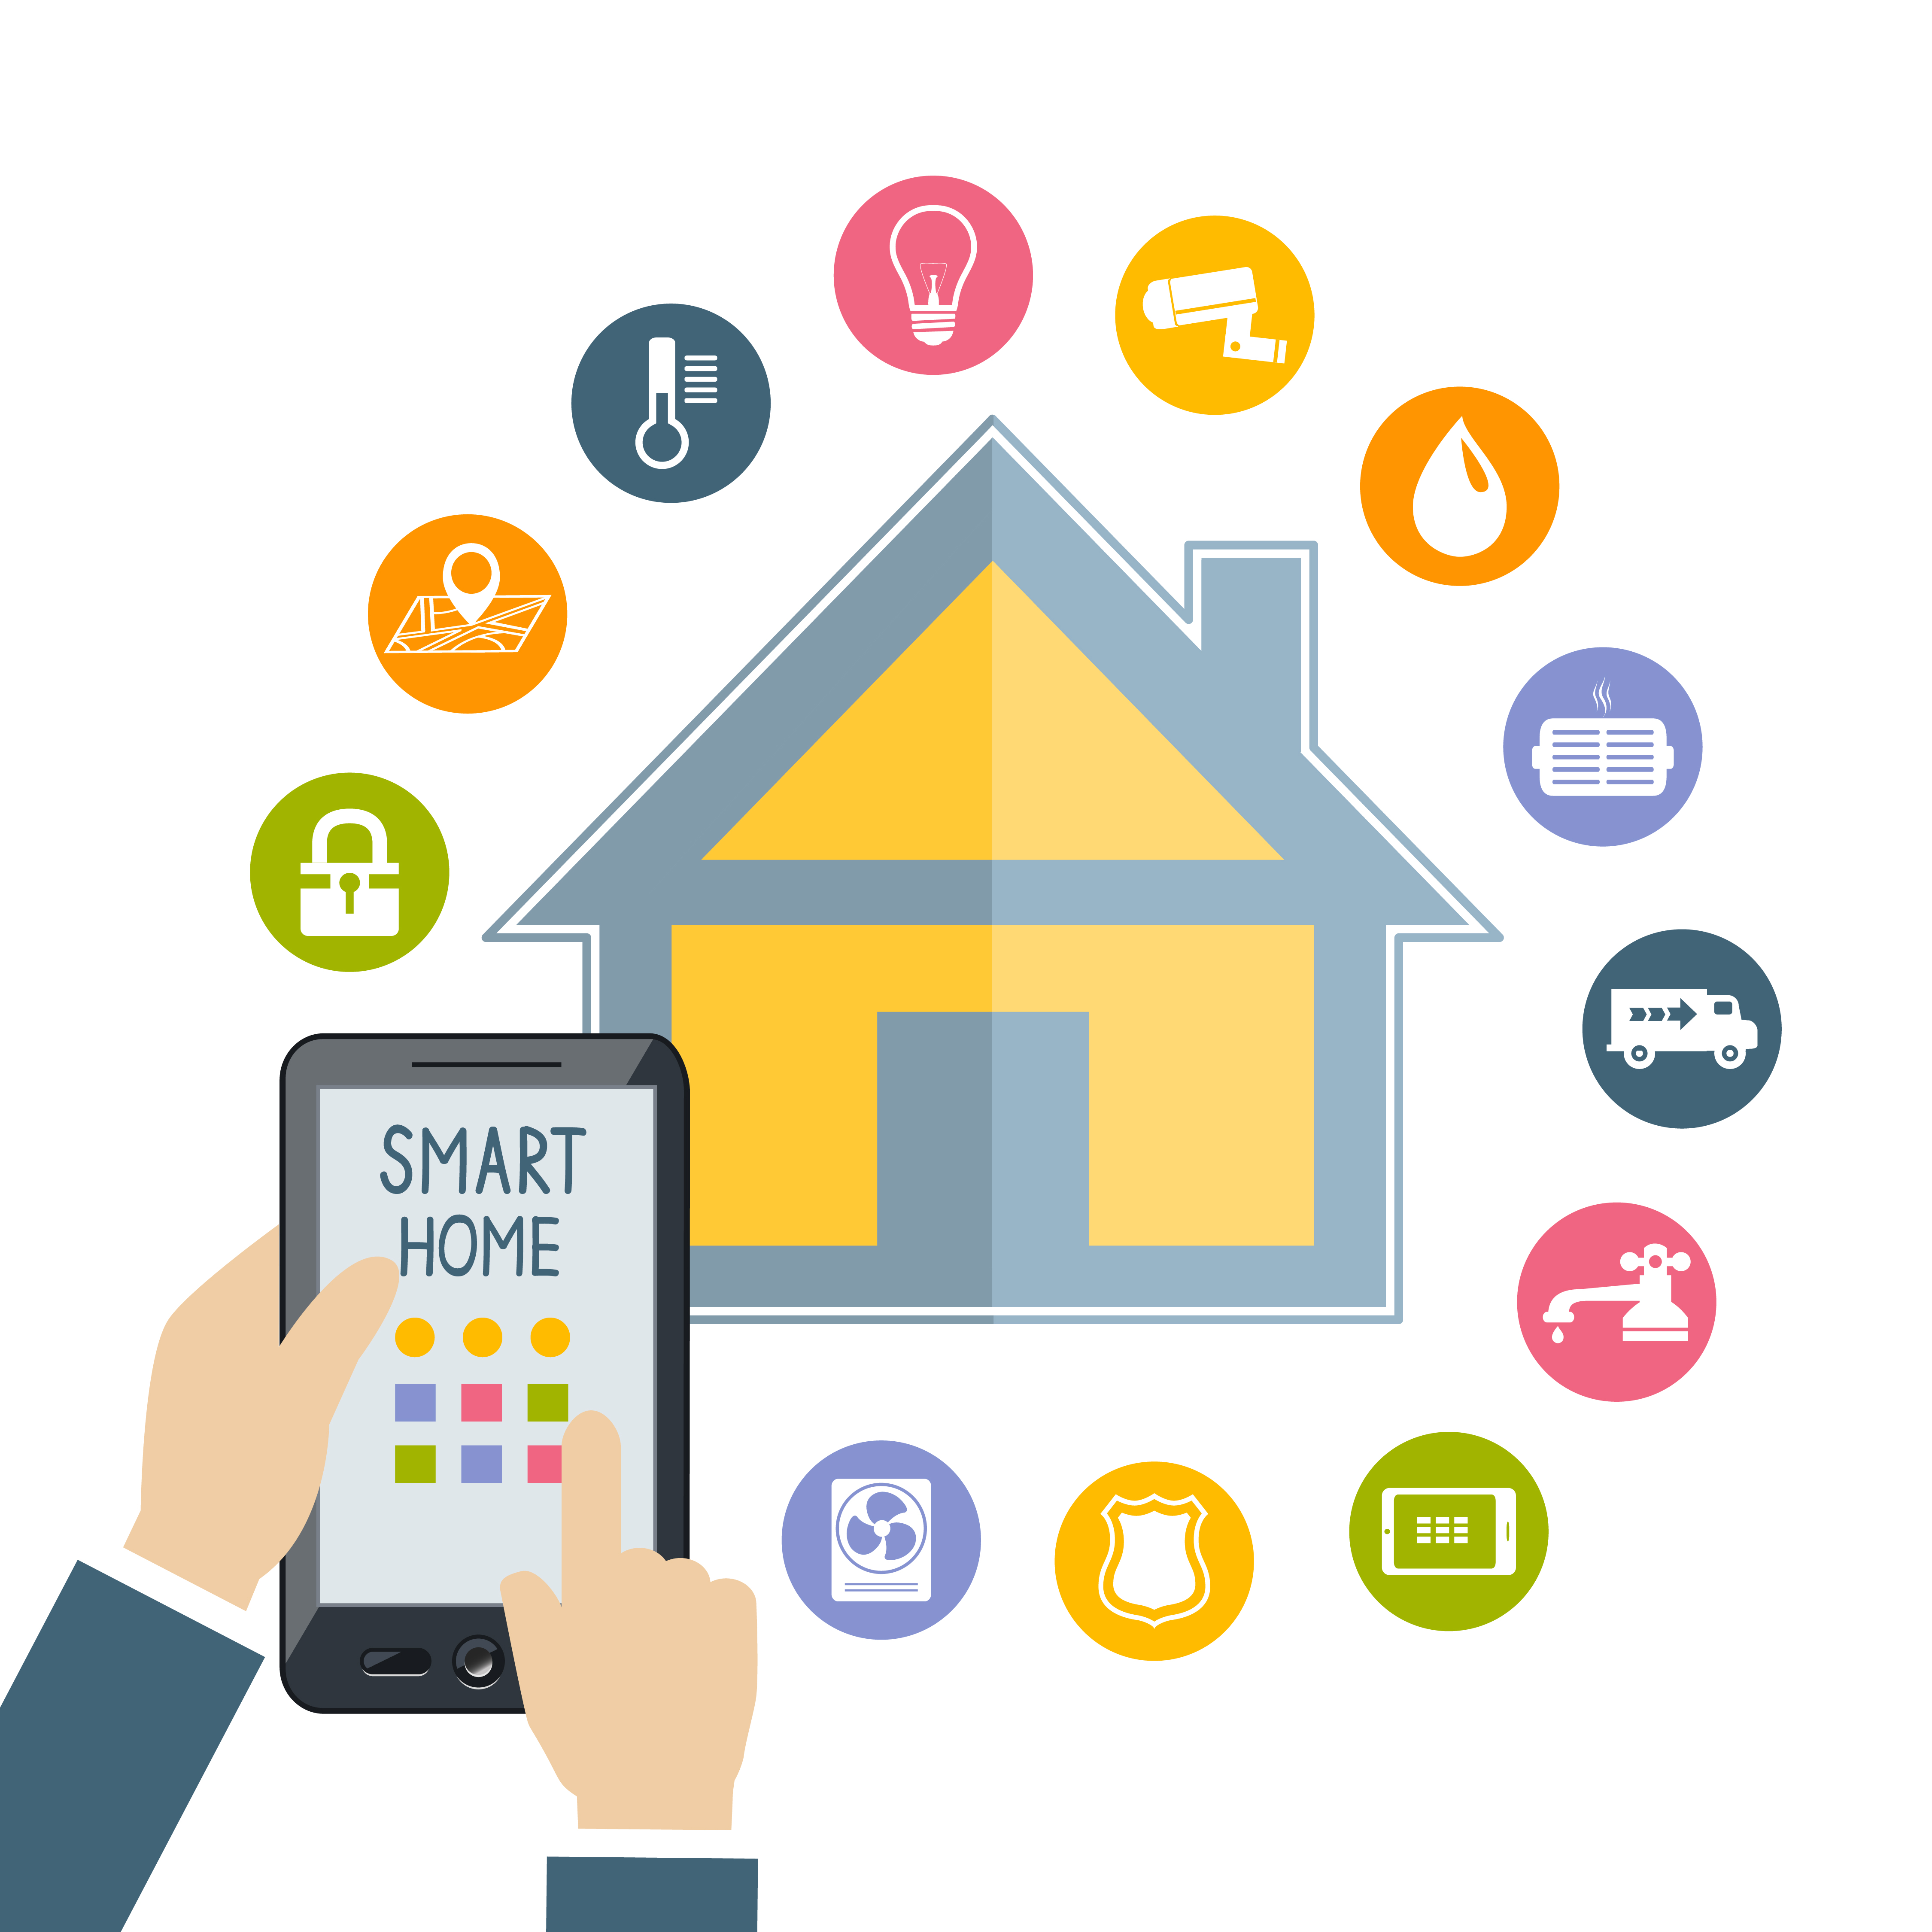
\includegraphics[scale=0.75]{98_Bilder/03_Marktsegmente/smarthome}
  \caption[Smart Home Symbolbild]{Smart Home}
  \footnotesize Quelle: \url{http://icon.asid.org/wp-content/uploads/2014/11/40349344_thumbnail.jpg}, Stand: 05.11.2015
\end{figure}
\newpage

\subsection{Detailhandel}
Im Verkauf hat die Revolution schon teilweise begonnen. Die grossen Player in der Schweiz beginnen alle ihre Filialen mit WLAN auszustatten. Momentan bieten diese den WiFi Zugang gratis den Kunden an. Somit steht der Kommunikationskanal für das IoT im Markt bereit und die Kunden sind zur gegebenen Zeit bereits verbunden damit.
Weiter werden bereits Selbstbezahlkassen eingesetzt. Momentan werden zwei Modelle verfolgt. Eine Einkaufsart ist der Kunde wählt seine Produkte und scannt diese selber ein, bezahlt mit Karte oder Bar und verlässt das Geschäft. Die dem IoT nähreren Methode registriert sich die einkaufende Person sich beim Eingang an einem Terminal und rüstet sich mit einem mobilen Strichcodeleser des Marktes aus oder nimmt sein Smartphone als Scanner. Die Person liest alle Produkte mit dem Scanner ein und bezahlt beim verlassen des Ladens beim Bezahlterminal. Beim abmelden des Scanners wird der Kunde ermittelt und das Total eingefordert.\\
Ein weiterer Schritt ist hier alle Produkte mit einer RFID zu taggen, somit könnte der Kunde nur seine Kreditkarte registrieren, die Waren in den Warenkorb legen und die Filiale verlassen. Beim verlassen wird, durch die Information auf dem RFID Tag, gemerkt welche Waren mitgenommen wurden und die Kreditkarte wird automatisch belastet.
\begin{figure}[H]
  \centering
  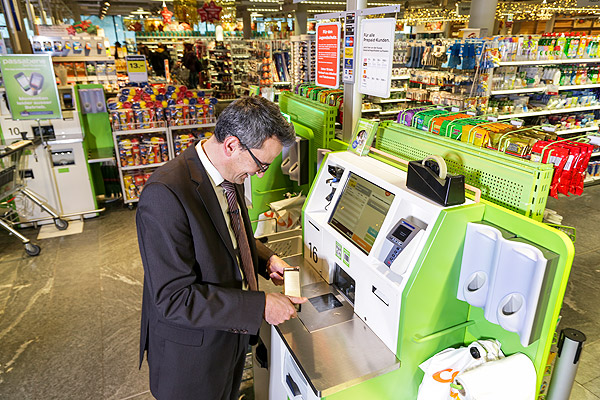
\includegraphics[scale=0.81]{98_Bilder/03_Marktsegmente/self_checkout}
  \caption[Self Checkout Kasse]{Eine Selbstbezahlkasse für mit mobilen Scanner oder zum selber einlesen}
  \footnotesize Quelle: \url{https://www.cooperation.ch/site/presse/get/12946772/Sutter-Selfscan_198B0923.jpg}, Stand: 05.11.2015
\end{figure}

\subsection{Mensch}
Der Mensch ist ein wichtiges Marktsegment, hierbei können Sensoren aller Arten den Menschen analysieren. Dieser Punkt wird bei der Marktsegmentierung Smartwatches und Smartwatche im Internet of Things genauer betrachtet.

\subsection{Natur}
Viele verschiedene Anwendungsfälle gibt es auch in der Natur. Es können Sensoren eingesetzt werden um Temperaturen, Luftdruck, Luftfeuchtigkeit oder Windstärke zu messen.  Mit Kombinationen von Sensoren, welche miteinander kommunizieren, können Frühwarnsysteme von Naturkatastrophen erschaffen werden. Dieses Segment hängt sehr nahe mit dem Marktsegement des Menschen zusammen.
\begin{figure}[H]
  \centering
  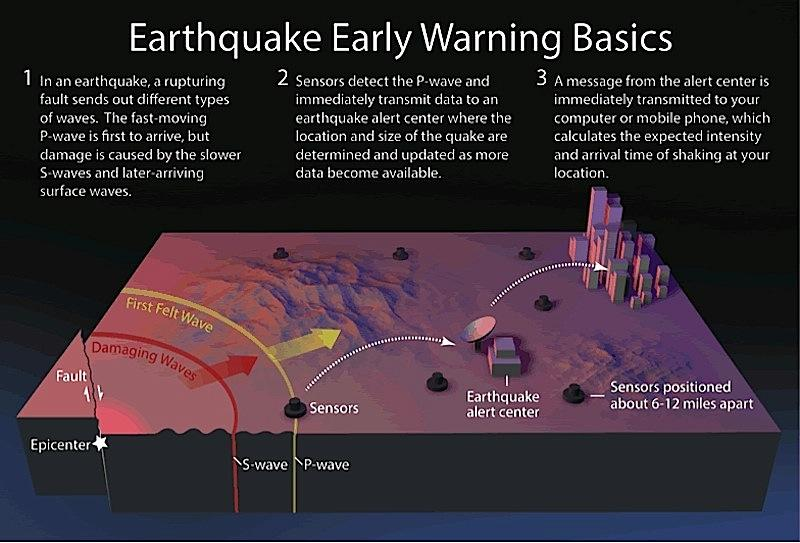
\includegraphics[scale=0.85]{98_Bilder/03_Marktsegmente/erdbeben}
  \caption[Frühwarnsystem von Erdbeben]{Wie ein Frühwarnsystem von Erdbeben funktioniert}
  \footnotesize Quelle: \url{http://www.ingenieur.de/var/storage/images/media/ingenieur.de/bilder/funktionsweise-fruehwarnsystems-shakealert/3666615-1-ger-DE/Funktionsweise-des-Fruehwarnsystems-ShakeAlert_image_width_884.jpg}, Stand: 05.11.2015
\end{figure}
\newpage

\section{Marktsegmente für Smartwatches}
\begin{tabbing}
xxxxxxxxxxxxxxxxxxxx\=xxxxxxxxxxxxxxxxxxxxxxxx	\kill
Mensch:		          \> Blutdruck, Puls, Bewegungen, Schlaf Überwachung, Lebensüberwachung, \\\>Sportbeobachtungen, Sporttracking \\
Zeit:			          \> Individuelle Zeitansichten, Zeitfunktionen \\
Benachrichtigung:	  \> Informationen am Handgelenk, Kommunizieren \\

Momentan werden Smartwatchs hauptsächlich zu Notifikationszwecke und Anlysen des Menschen genutzt. Noch ist das Potenzial nicht vorhanden um Smartwatches in vielen anderen Segmenten einzusetzen. Um dies zu ermöglichen muss das Umfeld zuerst geschaffen werden.
\end{tabbing}

\subsection{Mensch}
Heute werden Smartwatches verwendet, um den Menschen bei Aktivitäten überwachen zu können. Diese Wearables verfügen viele eingebaute Sensoren die die Bewegungen des Trägers analysieren und dem interessierten die Daten zur Verfügung stellen. Zu den Sensoren gehören z.B. ein Bewegungssensor, Schrittzähler, Herzfrequenzmesser und viele mehr.
Viele Hersteller von Smartwatches rüsten Ihre Produkte mit Sensoren und auch gleich Auswertungsapplikationen (z.B. Google Fit, Apple Health oder Motorola Moto Body).
Mit diesen Apps kann der User seine Daten gleich während dem Training auf der Uhr verfolgen oder später auf dem Smartphone auswerten. Dies macht zusätzliche Sport-/Pulsuhren überflüssig.

\subsection{Zeit}
Die Hauptaufgabe einer Uhr sollte es immernoch sein die Zeit genau anzuzeigen. Die Smartwatches haben die Möglichkeit nicht nur die aktuelle Uhrzeit anzuzeigen sondern auch als Weltuhr, Stoppuhr und Countdown Rechner zu fungieren. Dabei hat der Träger der Computeruhr die Wahl wie das Ziffernblatt aussehen soll, die Abbildung 3.10 verdeutlicht dies.
\begin{figure}[H]
  \centering
  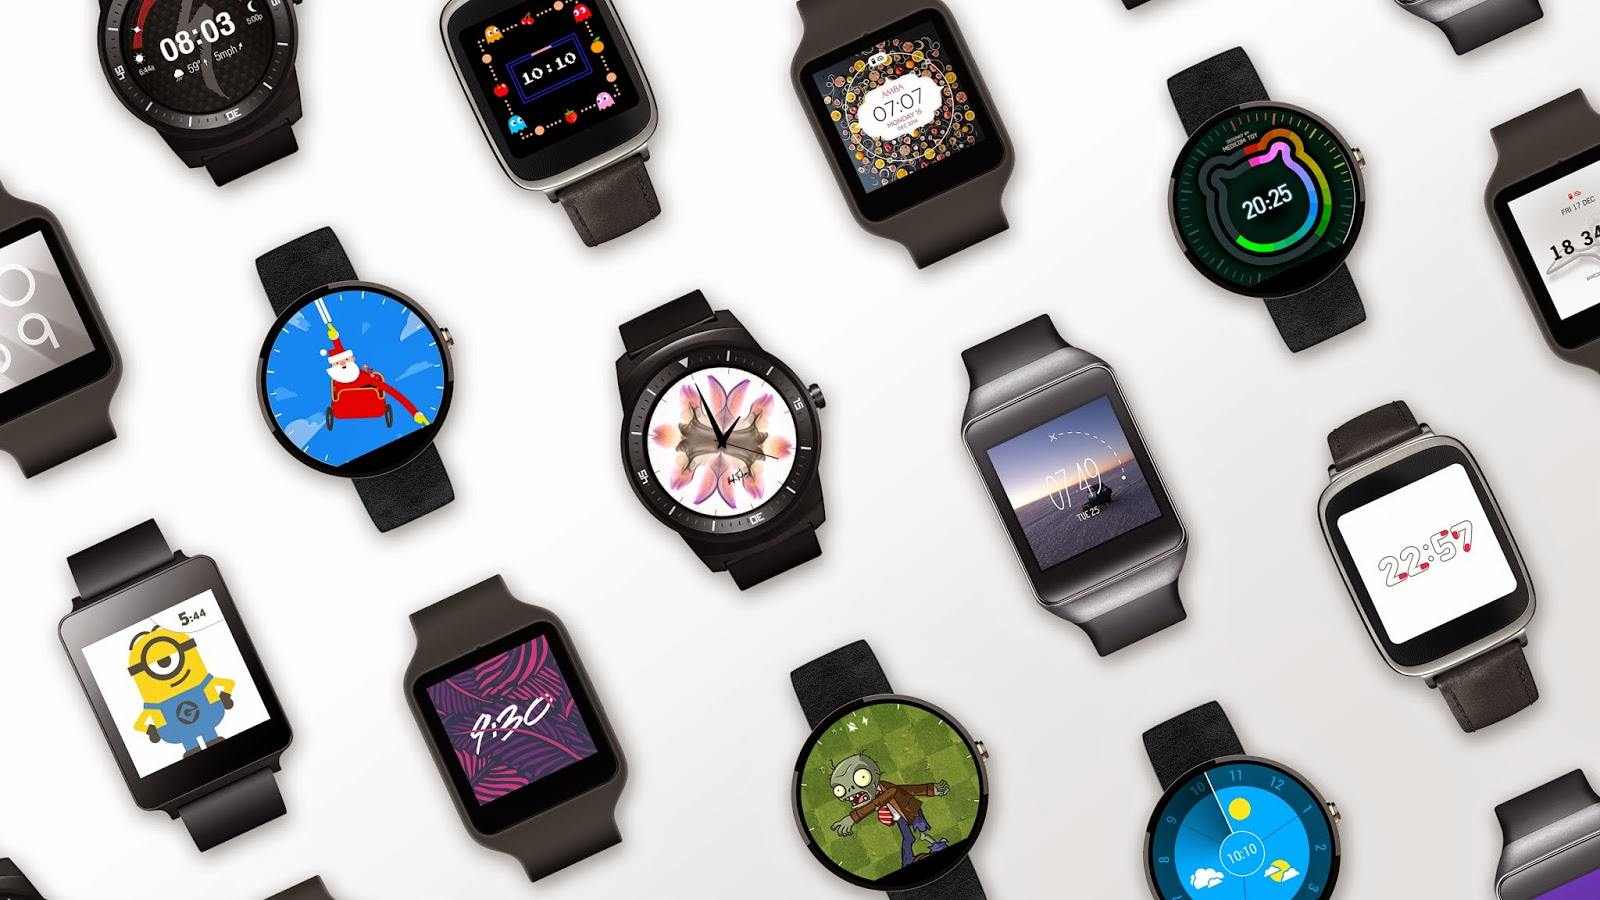
\includegraphics[scale=0.3]{98_Bilder/03_Marktsegmente/smartwatchfaces}
  \caption[Smartwatch Ziffernblätter]{Das Ziffernblatt der meisten Smartwatches kann individuell gestaltet werden}
  \footnotesize Quelle: \url{http://i1-news.softpedia-static.com/images/news2/Google-Launches-Watch-Face-API-You-Can-Customize-Your-Smartwatch-467130-2.jpg}, Stand: 12.11.2015
\end{figure}

\subsection{Benachrichtigung}
Eine Smartwatch wird neben der Uhrzeitfunktion auch als Notifikationsbildschirm verwendet. Alle relevanten Benachrichtigung an ein Smartphone können auch von der Smartwatch angezeigt werden. Dabei dient die Uhr meist als verlängerter Arm der Mobilgerätes. Es können Nachrichten empfangen, Telefonate geführt, Erinnerungen ausgelöst, der Wecker gestellt werden oder anzeigen was auf dem Smartphone ausgeführt wird (Siehe Abbildung 3.11).
\begin{figure}[H]
  \centering
  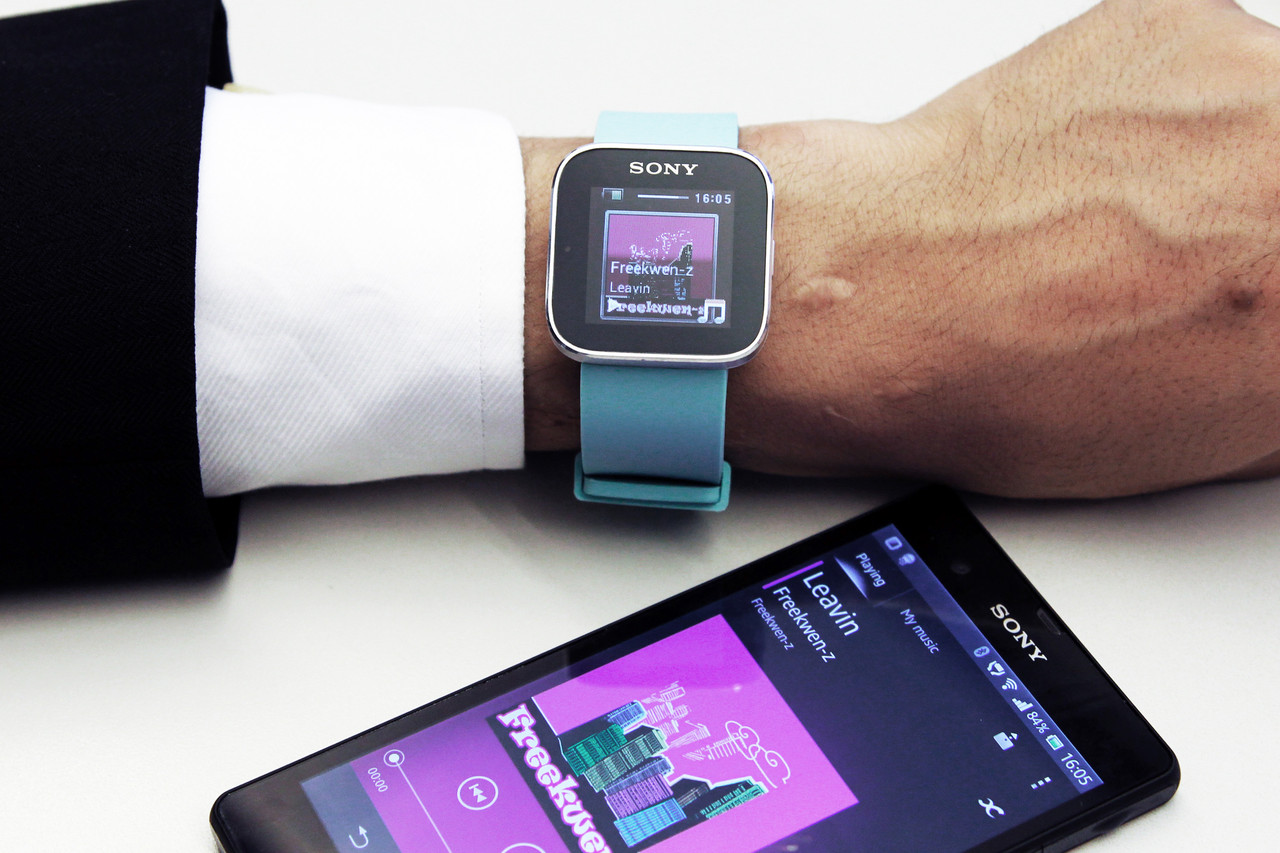
\includegraphics[scale=0.38]{98_Bilder/03_Marktsegmente/notifications}
  \caption[Smartwatch Anzeige von Smartphone]{Die Smartwatch zeigt an, welches Musikstück auf dem Smartphone abgespielt wird}
  \footnotesize Quelle: \url{http://smartwatchpro.it/wp-content/uploads/2015/08/OB-YT760_smartd_M_20130904020012.jpg}, Stand: 12.11.2015
\end{figure}
\newpage

\section{Marktsegmente für Smartwatches im Internet of Things}
\begin{tabbing}
xxxxxxxxxxxxxxxxxxxx\=xxxxxxxxxxxxxxxxxxxxxxxx	\kill
Mensch:		        \> Blutdruck, Puls, Bewegungen, Schlaf Überwachung, Gesundheitsbenachrichtigung \\
Benachrichtigung:	\> Chat, Telefonieren, Videotelefonie \\
Heimautomation:	  \> Fernbedienung, Statusanzeigen, Alarming \\
Detailhandel:		  \> Geldbörse, Produktebezeichnung, Einkaufsliste \\
Ortsbezogen:		  \> Navigation, Ortsspezifische Informationen, Ortung, Personen in der Nähe \\
\end{tabbing}

\subsection{Mensch}
